\documentclass[10pt]{amsart} 
\usepackage{graphicx} 
\usepackage{float} % necessary for placement of figures
\usepackage{amsmath}
\usepackage{tikz}
\usepackage{pgfgantt} % load Gant chart package
\usepackage{array}
\usepackage[style = authoryear, sorting = nyt, backend = biber]{biblatex}
\addbibresource[location = local, type = file]{C:/Users/bloh356/Google Drive/Library/Library.bib}
% \addbibresource[location = local, type = file]{/Users/bloh356/Google Drive/Library/Library.bib}


\graphicspath {{figures/}}

\title{Uncertainty in reliability parameter estimates: Inclusion in the Generation Expansion Planning (GEP) problem}
\author{Andrew Blohm}
\date{\today}

\begin{document}
\maketitle

\section{Abstract}
What does uncertainty and nonstationarity in gas-fired generator reliability mean for the long-term reliability of our electricity system (and its optimal design)(In progress)? 
We anticipate that traditional methods significantly underestimate the riskiness of investment decisions and thus, overestimate system reliability, which potentially exposes consumers, generators, and system operators to greater risks of unmet demand. 
The contribution of our model to the literature is in the assessment of uncertainty and nonstationarity of the outage rate parameter on the optimal resource mix (as compared to existing methods). 
We anticipate that the composition, costs, and reliability resulting from our method will be quite different than existing methods, which rely on single point parameter estimates. 

\section{Introduction}
Investments in energy production capacity are subject to partial or complete irreversibility (i.e., large, sunk cost that is not particularly fungible) and are large, high-risk investments facing uncertain operating environments (i.e., economic and regulatory uncertainty)\parencite{bakirtzis:2012aa}. 
The Generation Expansion Planning (GEP) problem has been employed extensively to manage these risks while selecting an optimal production portfolio. 
The GEP model determines how best to meet expected future demand through the selection of plant size, production technology, and location, as well as timing over a planning horizon, usually between 10 - 30 years \parencite{hemmati:2013ab}. 
The GEP problem is well studied, from a variety of perspectives including: solution algorithms, incorporation of new production technologies, uncertainty characterization, reliability, time horizon, etc. \parencite{hemmati:2013ab}.

Two approaches are generally used to determine the solution to the GEP: either a centralized or decentralized approach \parencite{bakirtzis:2012aa}.\footnote{The micro-approach incorporates a high amount of model complexity that require operations research or meta-heuristic methods to solve but with the caveate that there is no guarantee that global optimality is achieved. Macro-modeling approaches reduce complexity by ignoring those features and constraints.} 
The centralized approach is appropriate in monopoly situations (i.e., a monopoly utility determining least cost expansion plans) or in deregulated markets by governing or regulating authorities to better design markets and policies \parencite{bakirtzis:2012aa}.
Solution methods for the centralized problem include stochastic dynamic programming (SDP)\parencite{}, non-linear programming (NLP)\parencite{}, evolutionary programming \parencite{}, multi-objective programming \parencite{}, mixed-integer linear programming (MILP) \parencite{}, in addition to other approaches \parencite{}\parencite{bakirtzis:2012aa}.  
[Insert the citations from \cite{bakirtzis:2012aa}.]\footnote{The decentralized approach accounts for the behavior of market participants, usually in a deregulated market framework \parencite{bakirtzis:2012aa}. 
For a more detailed discussion of the decentralized approach the reader is directed to \cite{bakirtzis:2012aa}.} 

Uncertainty incorporation in the generation expansion planning problem has included price volatility, reliability of generation units, load forecast, electricity prices, and costs (i.e., fixed and variable) of each power production technology \cite{hemmati:2013ab, pereira2010decision, pereira2011generation}. 
However, to date, the literature is bereft of an analysis of the effect of uncertainty or trends in the forced outage rate (FOR) parameter on the optimal investment portfolio in the GEP problem. 
Past studies have demonstrated that small changes in the FOR can have significant effects on the reliability of the system \parencite{} (Shirvani (2012))[add citation]. 

There are significant, ongoing changes to the role and deployment of gas-fired generators that are potentially leading to changes in unit reliability. 
Natural-gas fired generators are more frequently ramping, as a result of more renewables, which is having unknown consequences but presumed negative affects on maintenance and reliability [add citation].
At the very least, generators are experiencing increasing O\&M costs as a result of increasing power plant cycling given larger deployments of variable generation, especially for plants designed as baseload units \parencite{nrel:2012aa}.\footnote{Cycling means operating the plant in response to system load requirements (i.e., load following, varying load levels, etc.); as opposed to operating it as a baseload resource \parencite{nerc:2012aa}. Each cycling exposes equipment to pressure and thermal stresses that can damage equipment and subsequently, lead to shorter component life expectancies, higher equivalent forced outage rates (EFOR), and shorter life expectancies \parencite{nerc:2012aa}.} 
These affects are being overlooked by current GEP problem formulations.

Power system adequacy in GEP problems has historically been addressed using deterministic methods, however, over the past few decades probabilistic criteria have largely replaced them.
Deterministic criteria include a planning reserve margin, which could be one of several measures including, setting the reserve margin to the size of the largest generation unit, percentage of system capacity, etc. 
The issue with deterministic approaches (e.g., planning reserve margin) is that they do not account for stochasticity in unit behavior, unit size, etc.
As a result, deterministic methods can lead to either over-investment or inadequate system reliability \parencite{aghaei:2013aa}.

Instead, stochastic methods naturally account for randomness such as unit forced outage rates, size, etc. but at the expense of an increasing computational burden \parencite{aghaei:2013aa}.  
In general, probabilistic metrics measure the duration, intensity or frequency in which demand exceeds the resources available at that time \parencite{dragoon:2006aa}.  	
The adequacy of the deployed resources to meet demand can be incorporated into the GEP problem using: Loss of Load Expected (LOLE)\footnote{The LOLE is the expected number of hours in which demand is not satisfied and is calculated as $LOLE = \sum_{k=1}^S P_k\left(C_T - L_k \right)\times t_k$, where there are S sub-periods and each sub-period is of length $t_k$.}, Loss of Load Probability (LOLP)\footnote{The LOLP is the long-run probability of power system demand exceeding the capacity available \parencite{endrenyi:1978}.  
LOLP can be calculated using daily peak load (i.e. hour demand for a 24 hour period) or using daily peak loads for a 1-year period using a load duration curve \parencite{endrenyi:1978}.}, Loss of Load Cost (LOLC), and Expected energy not served (EENS)\footnote{EENS is the expectation of the energy that the system is not capable of serving and is calculated as the following $EENS = P_k \left(C_T - L_k \right)\times \left(C_T- L_k \right)$.}.\footnote{Given its simplicity LOLE has been extensively used in the past, however, EENS does have certain advantages including that it encompasses the degree of the deficiency, as well as the likelihood \parencite[p622]{murugan2009nsga}.}

In this paper the centralized GEP problem is formulated as a two-stage stochastic mixed integer program.
In the first stage the model makes investment decisions while in the second stage the model checks to see that the system meets reliability constraints while in operation. 
We consider the forced outage rate of each plant as a random variable, which necessarily impacts system reliability. 
The reliability metric (i.e., LOLE, LOLP, EENS, etc.) are highly sensitive to the EFOR parameter (i.e., a small change in the parameter estimate can lead to large changes in the reliability metric. 
GEP models have not explored the solution space that surrounds the EFOR parameter estimate. 

The rest of this paper is organized as follows: in the second section we discuss the data used in the analysis. 
In the third section, we discuss existing methods for incorporating uncertain parameters, including the forced outage rate, into an optimization framework.
In the fourth section, we propose the mathematical formulation of the two-stage stochastic mixed integer problem. 
In the fifth section, we introduce our case studies before we discuss the results of our model formulation.
In the final section, we discuss some relevant conclusions of our work. 

\section{Data}
The proposed model is evaluated using the IEEE 14 and 30 bus test system \parencite{christie:2009aa}.\footnote{We downloaded the power system data for each of the 14, 30, 57, 188, and 300 bus test systems.}  
[Talk with Jeremy about the appropriate test system].


\section{Methods}
The GEP problem is a large-scale, highly-constrained mixed-integer linear program (MINLP) that requires complete enumeration (i.e., investigation of every combination of assets over the time horizon) to identify the global optimum \parencite{bakirtzis:2012aa}.  
The inability to undertake such an exercise has led to the development of simplifications to reduce the computational load of the problem. 

A common approach to dealing with uncertainties in the GEP framework is Monte Carlo methods \parencite{pereira2010decision}.
Typically, the LOLE and EENS are generated using Monte Carlo techniques \parencite{billinton1996reliability, li2012uncertainty}. 
It is typically built recursively using the Capacity Outage Cumulative Probability Table (COCPT).\footnote{COCPT assumes that the failure of a unit is ``independent of the operating level, system load, and the outage pattern of other units'' (Goel presentation, 2011).} 

Assessing system adequacy using stochastic methods can lead to computational issues given the widely held belief that the GEP is actually a mixed integer non-linear program \parencite{aghaei:2013aa}.
As a result, several methods were developed to assess system adequacy.
\cite{} proposed the 'Z-Method' to evaluate system adequacy in the GEP problem, which replaces the stochastic adequacy assessment metric (i.e., loss-of-load probability (LOLP)) with a new constraint. 
The approach accounts for unit forced outage rates (FOR), system adequacy targets\footnote{In the GEP formulation framework the modeler would select an acceptable level of service (i.e., industry standard is an insufficient capacity with a frequency of 1-in-10 years)\parencite{}. 
The model would then calculate the appropriate reliability statistic using the EFOR (i.e., the number of hours of unit failure as a percentage of all available hours) for each generation unit type and size.}, uncertainty in expected load growth, as well as the size, type and number of units in the production mix \parencite{aghaei:2013aa, \ldots}. 

\section{SMIP GEP problem formulation}
\subsection{Objective function \nopunct}

\subsection{Constraints \nopunct}
\subsubsection{Maximum construction limit \nopunct}
This constraint is a maximum allowable number, capacity, or investment amount for new generation sources to be built during period \textit{t} given limited resources (i.e., capital, manpower, space, etc.). 
\subsubsection{LOLP constraint \nopunct}
\begin{equation}
\textit{lolpc}_{t} \leq \textit{lolps}_{t} \forall t \in T 
\end{equation}

The $\textit{lolpc}_{t}$ is the loss-of-load probability at stage \textit{t} and $\textit{lolps}_{t}$ is the loss-of-load probability limit (i.e., the reliability target selected by the user) \parencite{dragoon:2006aa}. 
The equivalent Z constraint is \ldots


\subsubsection{Non-negativity constraints \nopunct}

\section{\ldots [Name of solution algorithm}


As a result, 
Planning and investment in power generation capacity expansion is difficult given the competing objectives for power producers (i.e. minimization of investment costs and maximization of reliability); uncertainty in a number of parameters (i.e.\ costs, demand, regulation), physical and technical constraints, complex mix of regulated and deregulated market structure across the country, and, large and lumpy investments, to name a few. 
One tool used in the long-term power planning process is Generation Expansion Planning (GEP) problem, which provides a framework to optimize generation investment.
	
\section{SMIP GEP: Case study}
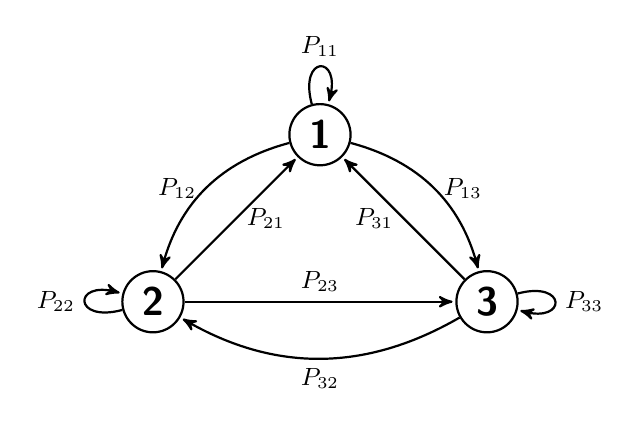
\begin{tikzpicture}[->,>=stealth',shorten >=1pt,auto,node distance=3cm,
                    thick,main node/.style={circle,draw,font=\sffamily\Large\bfseries}]
	\node[main node](1){1};
	\node[main node](2)[below left of=1]{2};
	\node[main node](3)[below right of=1]{3};

	\path[every node/.style={font=\sffamily\small}]
	 (1) edge [bend left] node[right] {$P_{13}$} (3)
	 edge [bend right] node[left] {$P_{12}$} (2)
	 edge [loop above] node[above] {$P_{11}$ }(1)
	 (2) edge node [right] {$P_{21}$} (1)
	 edge node [above] {$P_{23}$} (3)
 	 edge [loop left] node[left] {$P_{22}$} (2)
	 (3) edge node [left] {$P_{31}$} (1)
	 edge [loop right] node[right]{$P_{33}$} (3)	
	 edge [bend left] node[below]{$P_{32}$}(2);
\end{tikzpicture}

	
	
	
	
	
	
	
		
\subsection{Data}	
One approach would be to test the methods on the IEEE Reliability Test system \parencite{billinton:1994aa}. 
We use the IEEE Reliability Test System as an example system topology \parencite{}. 

	The changing electricity generation mix requires that industry personnel gain more experience with ``generating resource technology behavior, operating characteristics, and optimal planning approaches in order to properly assess reliability or improve performance analysis'' \parencite{nerc2011gads}. 
	Understanding the reliability and performance of existing and new production technologies is necessary to understand the reliability of the bulk power system in North America \parencite{nerc2011gads}. 
	It is also important to electric utilities since poor performing units can result in higher operating costs (i.e., loading units out of economic order), a need to purchase power, and/or installing additional capacity \parencite{}(GADS Introduction material).
	The industry, as a result, created the Generating Availability Database (GADs) as a means to share information on the causes and effects of unavailability, in addition to the development and improvement of strategies to prevent or mitigate availability losses that have proven useful to others \parencite{}(GADS intro material). 
	
	The North American Electric Reliability Corporation (NERC) compiles the Generating Availability Data System (GADS), which is an annual summary report for power stations located in the United States and Canada \parencite{nercgads}. 
	GADS contains information about the type of equipment used, performance characteristics, and descriptions of events (i.e. equipment failures). 
	Four types of events are reported in GADS: outages, deratings, reserve shutdowns, and non-curtailing events \parencite{gugel2015polar}. 
	It also contains data on the reliability, availability and maintainability of power plants (i.e., outage data). 
	The dataset includes the equivalent forced outage (EFOR), which is defined as the hours of unit failure (i.e. unplanned outage hours and equivalent unplanned derated hours) as a percentage of total available hours (i.e. unplanned outage, unplanned derated, and service hours)(wikipedia, GADS).\footnote{EFOR is calculated using IEEE Standard 762 definitions \parencite{gugel2015polar}.} 
	Outages can be divided into planned -- scheduled maintenance, versus unplanned outages -- unscheduled outages. 
	
	GADS began in 1979 as an extension of a data collection process that begin during the 1960s \parencite{}(GADS, The generating availability data system (GADS): Application and benefits, 1995).
	The database began as a voluntary with each participating utility providing detailed reports of each units operation and performance.
	However, since January 1, 2013, it is mandatory for conventional generating units with a nameplate capacity $\geq$ 20 MW to report reliability information to GADS \parencite{}(GADS frequently asked questions).  
	Variable energy sources are not required to report reliability information; a taskforce is currently underway to assess the best data collection methods for solar \parencite{}(GADS frequently asked questions). 
	The reports include quarterly information on the design information, types of outages and deratings, energy produced, fuel use, etc., which are then summarized in the annual \textit{Generating Availability Report} \parencite{} (GADS, The generating availability data system (GADS): Application and benefits, 1995).   
	It has involved to include data collection, data maintenance and support, in addition to data processing and reporting (i.e., trends in industry availability).
	
	The GADS contains operating histories for more than 7,700 generating units located in North America ($\approx$ 90\% of all installed generating capacity)\parencite{}(Generating Availability Data System: Data Reporting Instructions, 2015). 
	Events are defined as any time the operating status of a generator changes and include: outages, derates, reserve shutdowns, and non-curtailing events \parencite{}(Generating Availability Data System: Data Reporting Instructions, 2015).
	The event report will include informaiton on the event magnitude, primary cause, and, additional causes or components worked during the event \parencite{}(Generating Availability Data System: Data Reporting Instructions, 2015, pIII-2).
	In Figure \ref{fig:unit.states.GADS} we show the Unit States diagram from the \parencite{}(Generating Availability Data System: Data Reporting Instructions, 2015, pIII-5).
	

	Resources can first be categorized by whether they are active or inactive.
	Inactive resources are in one of three potential states: inactive reserve (IR), mothballed (MB), and, retired (RU). 
	An inactive reserve, mothballed, or retired unit is a unit whereby the unit is unavailable for an extended period of time for reasons unrelated to the equipment \parencite{}(Generating Availability Data System: Data Reporting Instructions, 2015, pIII-5). 
	Active states include: available and unavailable, which can be further broken down into unplanned outages and planned deratings for available resources, as well as unplanned outages and planned outages for unavailable resources \parencite{} (Generating Availability Data System: Data Reporting Instructions, 2015, pIII-6). 
	``An outage exists whenever a unit is not synchronized to the grid system and not in a reserve shutdown state. 
	An outage starts when the unit is either desynchronized from the grid or when it moves from one unit state to another (for example, goes from a reserve shutdown to a maintenance outage). 
	The outage ends when the unit is synchronized to the grid or moves to another unit state'' (Generating Availability Data System: Data Reporting Instructions, 2015, pIII-6). 
	
	In the GADS database an interruption in fuel supply, for example, as a result of interruptible supply of fuel as part of a fuel contract would be considered as events caused by external economic factors with a cause code 9131 \parencite{} (Generating Availability Data System: Data Reporting Instructions, 2015, Appendix B - pB-FS-29). . 
	
	The underlying data, used to calculate the annual summaries, is not publically available.
	Data sharing in GADS works via the following mechanism: an electric utility would share information for the types of power plants in its portfolio of assets.
	In GADS it would then have access to more detailed (and not publically available) reliability information concerning only those types of power plants.   
	The Generating Availability Report contains 17 categories of statistics for generating units and related equipment, which can be viewed at an annual or five-year cumulative basis. 
	The generating units are grouped by type, size (i.e., nameplate rating), and fuel (i.e., primary fuel used). 
	 
\subsection{Methods}
	We propose to use the GADS dataset to build a Bayesian regression model to estimate a posterior distribution around the EFOR parameter for each type (and size grouping) of power plant. 
	Reliability is known to be a function of or at least correlated with the size and type of power plant. 
	In our regression model we will control for confounding factors (i.e., weather, location, etc.) and trends (i.e., capacity factor, etc.) in the dataset.  
	
	Each generation unit can be represented by its capacity and its unavailability and each unit has only two states: on or an outage. 
	One disadvantage of the model is that it is a two-state system (i.e. up or down) while generating units are necessarily more complex in that they may experience partial failures in which they operate at reduced capacity levels (i.e. a 3- or even multi-state model).
	The capacity is a random variable in reliability analysis (Phoon, 2006, p19).
	\[
 	   P(X=x_i)=\left\{
             		   \begin{array}{c l}
             			   1-q & x_i = capacity_i \\
             			   q & x_i = 0
            		    \end{array}
         			\right.
	\]
	where, $q$ is the equivalent forced outage rate (EFOR)
	The capacity out of service then is multinomially distributed. 
	There are $2^n$ possible states, where $n$ is the number of generating units.
	And the likelihood of capacity greater than a particular value is $P(X \geq x_k) = \sum_{i \geq k} p(x_i)$.
	In other words, we sum all of the outcomes in which capacty exceeds a particular value and repeat this from the smallest unit capacity to the total system capacity value.  
	The likelihood of different capacity outages of the system, which is the basis of the COCPT. 			
	

\printbibliography
\end{document}

